\documentclass[11pt,a4paper]{article}

% Encodage et langues
\usepackage[utf8]{inputenc}
\usepackage[T1]{fontenc}
\usepackage[french]{babel}

% Mathématiques et symboles
\usepackage{amsmath}
\usepackage{graphicx}
\usepackage{caption}
\usepackage{subcaption}
\usepackage{geometry}
\usepackage{newpxtext}
\usepackage{newpxmath}
\usepackage{microtype}
\usepackage{csquotes}
\usepackage{hyperref}
\usepackage{cleveref}
\usepackage{listings}
\usepackage{tcolorbox}
\usepackage{float}
\usepackage{placeins}

% Configuration des marges
\geometry{left=2.5cm,right=2.5cm,top=2.5cm,bottom=2.5cm}

% Configuration des liens
\hypersetup{
    colorlinks=true,
    linkcolor=blue,
    filecolor=magenta,      
    urlcolor=cyan,
    citecolor=red,
    pdftitle={SiraEdge - Module d'Optimisation de Portefeuille},
    pdfauthor={Ismail Moudden},
    pdfsubject={Optimisation de Portefeuille Quantitative},
    pdfkeywords={finance, optimisation, portefeuille, machine learning, risk parity}
}

% Configuration des listings
\lstset{
    basicstyle=\ttfamily\small,
    breaklines=true,
    frame=single,
    numbers=left,
    numberstyle=\tiny,
    showstringspaces=false,
    tabsize=2,
    captionpos=b
}

% Configuration des tcolorbox
\tcbuselibrary{skins}
\tcbset{
    enhanced,
    colback=blue!5,
    colframe=blue!75!black,
    fonttitle=\bfseries,
    boxrule=0.5pt
}

% Macro pour gérer les figures manquantes
\newcommand{\maybeincludegraphics}[2][]{%
    \IfFileExists{#2}{\includegraphics[#1]{#2}}{\fbox{Figure manquante: #2}}
}

% Chemin des figures
\graphicspath{{../figures/}{../../}}

\begin{document}

\title{\textbf{SiraEdge - Module d'Optimisation de Portefeuille}\\[0.9em]
\large{Recherche et Implémentation de Modèles Quantitatifs}}

\author{Ismail Moudden\\[0.6em]
\textit{SiraEdge — Module d'Optimisation de Portefeuille}}

\date{\today}

\begin{titlepage}
\thispagestyle{empty}
\maketitle
\vspace{2em}

\begin{abstract}
Ce rapport présente le module d'optimisation de portefeuille développé pour la plateforme SiraEdge, une solution innovante visant à démocratiser l'accès aux outils professionnels de gestion d'actifs. Nous détaillons l'implémentation, l'analyse comparative et la validation de sept modèles d'optimisation : Markowitz, Risk Parity, Monte Carlo, Black-Litterman, Machine Learning, Hybride et Métriques Personnalisées. L'étude inclut une analyse walk-forward robuste et une évaluation des performances sur données réelles (2020-2023). Tous les codes sources, figures et résultats sont disponibles dans le repository GitHub associé.
\medskip\par\noindent\textit{Portée.} Ce document est un \textbf{rapport technique et pédagogique} montrant le fruit des recherches et implémentations; il ne constitue \emph{ni une recommandation d'allocation}, \emph{ni une promesse de performance future}.
\end{abstract}

\vfill
\end{titlepage}

\section*{Contexte et Vision de SiraEdge}

\subsection*{Notre Mission}
SiraEdge est né d'une vision simple mais ambitieuse : \textbf{démocratiser l'accès aux outils professionnels de gestion de portefeuille}. Notre mission est de rendre la finance accessible à tous, en combinant rigueur mathématique et expérience utilisateur intuitive.

\subsection*{La Plateforme SiraEdge}
SiraEdge est une plateforme interactive développée pour apprendre à investir et simuler des portefeuilles. Elle intègre plusieurs modules :
\begin{itemize}
    \item \textbf{Simulation de Portefeuilles} : Test de stratégies sans risque
    \item \textbf{Module d'Optimisation} : Ce rapport présente ce module
    \item \textbf{Apprentissage Interactif} : Tutoriels et ressources éducatives
    \item \textbf{Analyse de Performance} : Métriques et visualisations avancées
\end{itemize}

\subsection*{Contexte de ce Module d'Optimisation}
Ce document présente \textbf{le résultat concret d'un travail de R\&D et d'implémentation} des modèles d'optimisation intégrés à SiraEdge. L'objectif est \textbf{de montrer le fruit des recherches} (codes, figures, protocoles) et de fournir une base reproductible. Il ne s'agit pas d'une note de recommandation, mais d'un \emph{rapport technique et pédagogique}.

\begin{itemize}
    \item Mettre à disposition des scripts prêts à l'emploi pour générer les figures
    \item Comparer les modèles sur un univers de test cohérent (2020--2023)
    \item Expliquer les compromis risque/rendement et les limites pratiques
    \item Documenter les choix d'hyperparamètres et le protocole de backtest
\end{itemize}

\subsection*{Positionnement dans l'Assistant IA SiraEdge}
Dans SiraEdge, l'assistant IA est \textbf{un chatbot d'aide et d'analyse} : il répond aux questions des utilisateurs, explique les figures et \textbf{analyse les stratégies} avec les métriques disponibles (Sharpe, Sortino, Calmar, stabilité, turnover). Il peut comparer des modèles et interpréter les résultats, mais \textbf{il ne fournit pas de recommandation d'investissement personnalisée}. Les graphes et tableaux de ce rapport constituent sa base de connaissances technique.

\subsection*{Portée du rapport — ce que c'est / ce que ce n'est pas}
\textbf{Ce que c'est}
\begin{itemize}
  \item Un compte rendu de R\&D et d'intégration des modèles (Markowitz, Risk Parity, BL, ML, Hybride, etc.)
  \item Un support de l'assistant IA pour illustrer les concepts et les résultats
  \item Un protocole de backtest reproductible avec métriques normalisées
\end{itemize}
\textbf{Ce que ce n'est pas}
\begin{itemize}
  \item Une stratégie de trading clé en main ou une recommandation personnalisée
  \item Une étude marketing; les chiffres servent l'\emph{apprentissage} et la comparaison
  \item Un engagement de performance future; l'univers et la période sont de démonstration
\end{itemize}

\subsection*{Backtesting et statistiques dans SiraEdge}
Le moteur d'optimisation est relié au \textbf{module de backtesting} de SiraEdge. Les scripts produisent des séries de rendements et des tableaux de métriques (Sharpe, Sortino, Calmar, stabilité des poids, turnover) qui alimentent les pages \texttt{Statistiques} et \texttt{Simulation}. Les résultats sont présentés \textbf{à des fins comparatives et pédagogiques} et peuvent différer de performances futures; les chiffres dépendent de la période (2020--2023), de l'univers choisi et des hypothèses (coûts, contraintes).

\subsection*{Approche Pédagogique}
Notre approche combine :
\begin{itemize}
    \item \textbf{Rigueur Scientifique} : Implémentation fidèle des modèles académiques
    \item \textbf{Accessibilité} : Explications claires et exemples concrets
    \textbf{Reproductibilité} : Code source complet et documentation détaillée
\end{itemize}

\subsection*{Repository GitHub}
Tous les codes sources, scripts de génération des figures, et ressources de ce projet sont disponibles dans le repository GitHub :
\begin{center}
\textbf{\url{https://github.com/SiraEdge/portfolio-optimization}}
\end{center}

\textbf{Structure du Repository :}
\begin{itemize}
    \item \texttt{src/} : Implémentation Python de tous les modèles
    \item \texttt{figures/} : Graphiques et visualisations générés
    \item \texttt{rapport/} : Sources LaTeX de ce rapport
    \item \texttt{README.md} : Instructions d'installation et d'utilisation
    \item \texttt{requirements.txt} : Dépendances Python
\end{itemize}

\textbf{Note importante :} Ce rapport fait référence à des fichiers de code spécifiques. Pour une compréhension complète et la possibilité de reproduire les résultats, il est essentiel de consulter le repository GitHub associé.

\newpage

\tableofcontents

\newpage

\section{Introduction}
Ce rapport présente, dans un cadre pédagogique et reproductible, plusieurs approches d'optimisation de portefeuille: modèles classiques, méthodes alimentées par l'apprentissage automatique, variantes hybrides et optimisation par métriques personnalisées. Les figures sont générées par des scripts Python (dossier \texttt{src/}) et référencées ici.

\begin{tcolorbox}[title=Contexte et objectifs de recherche]
Ce document présente un cadre d'allocation de portefeuille conforme aux standards académiques: exposition formelle des modèles, hypothèses explicites, protocole expérimental, hyperparamètres, résultats et analyse critique. L'ambition est de produire un artefact \emph{reproductible} (scripts, figures, dépendances) et \emph{interprétable} (justification des choix et limites).
\end{tcolorbox}

\section{Notions et vocabulaire}

\subsection{Concepts fondamentaux de la finance}

\textbf{Portefeuille :} C'est simplement un ensemble d'actifs (actions, obligations, etc.) dans lequel on place son argent. Penser à un panier avec différents fruits - chaque fruit représente un actif, et la quantité de chaque fruit représente le poids de cet actif dans le portefeuille.

\textbf{Rendement :} C'est le gain ou la perte en pourcentage sur une période. Si tu achètes une action à 100€ et qu'elle vaut 110€ un an plus tard, le rendement est de 10\%. En finance, on utilise souvent les \emph{rendements logarithmiques} car ils s'additionnent mieux dans le temps.

\textbf{Volatilité :} C'est une mesure de l'instabilité du prix d'un actif. Plus un actif est volatil, plus son prix peut monter ou descendre rapidement. C'est comme une voiture qui roule vite - elle peut aller loin mais aussi déraper plus facilement.

\textbf{Corrélation :} Mesure à quel point deux actifs évoluent ensemble. Si deux actions montent et descendent en même temps, elles sont corrélées positivement. Si l'une monte quand l'autre descend, elles sont corrélées négativement. Une corrélation de 0 signifie qu'elles évoluent indépendamment.

\subsection{Outils d'analyse et de test}

\textbf{Backtest :} C'est comme "rejouer l'histoire" avec une stratégie d'investissement. On prend des données passées et on simule ce qui se serait passé si on avait appliqué notre stratégie à l'époque. C'est utile pour tester des idées sans risquer de l'argent réel, mais attention : le passé ne garantit pas l'avenir !

\textbf{Walk-forward :} Technique plus sophistiquée que le backtest simple. Au lieu de tester sur toute l'historique, on teste sur des fenêtres glissantes (par exemple, 252 jours = 1 année de trading). Cela simule mieux la réalité où on ne connaît que le passé pour prendre des décisions.

\textbf{Reéquilibrage :} Action de modifier les poids des actifs dans le portefeuille pour revenir à l'allocation cible. Par exemple, si l'objectif est 50\% actions + 50\% obligations, et qu'après un an les actions valent 60\% du portefeuille, on vend des actions pour acheter des obligations.

\subsection{Styles d'investissement}

\textbf{Défensif :} Stratégie qui privilégie la stabilité et la protection du capital plutôt que la performance maximale. On accepte des rendements plus faibles pour éviter les grosses pertes. C'est comme conduire prudemment sur une route glissante.

\textbf{Low turnover :} Stratégie qui limite les changements fréquents dans le portefeuille. Moins on bouge, moins on paie de frais de transaction. C'est comme un jardinier qui laisse ses plantes pousser plutôt que de les déplacer constamment.

\textbf{Core-satellite :} Approche qui combine deux stratégies : un "cœur" stable (core) qui représente la majorité du portefeuille, et une partie plus dynamique (satellite) pour tenter d'améliorer la performance. C'est comme avoir une maison solide (core) et un jardin d'agrément (satellite).

\subsection{Métriques de performance}

\textbf{Ratio de Sharpe :} Mesure l'efficacité d'un investissement en comparant le rendement excédentaire (par rapport au taux sans risque) à la volatilité. Plus il est élevé, mieux c'est. C'est comme mesurer combien de kilomètres on fait par litre d'essence - on veut le maximum de rendement pour le minimum de risque.

\textbf{Ratio de Sortino :} Similaire au Sharpe, mais ne pénalise que la volatilité "négative" (les pertes). C'est plus logique car on s'inquiète plus des pertes que des gains.

\textbf{Ratio de Calmar :} Compare le rendement annualisé au maximum drawdown (plus grande perte sur une période). Plus il est élevé, plus le portefeuille récupère vite ses pertes.

\textbf{Maximum Drawdown (MDD) :} Plus grande perte en pourcentage depuis un pic. Si ton portefeuille valait 100€, puis 80€, puis 90€, le MDD est de 20\% (de 100€ à 80€).

\textbf{Stabilité des poids :} Mesure à quel point l'allocation du portefeuille reste stable dans le temps. Des poids qui changent peu signifient moins de frais de transaction et une stratégie plus prévisible.

\textbf{Turnover :} Mesure l'activité de trading. Un turnover de 100\% signifie qu'on a échangé l'équivalent de 100\% de la valeur du portefeuille sur la période. Plus c'est élevé, plus les frais de transaction impactent la performance.

\subsection{Coûts et contraintes}

\textbf{Frais de transaction :} Coûts payés à chaque achat ou vente (commissions de courtier, spreads, etc.). En général exprimés en "points de base" (bps) : 1 bps = 0,01\%. Des frais de 5 bps signifient qu'on paie 0,05\% à chaque transaction.

\textbf{Contraintes de poids :} Limites imposées sur la part de chaque actif. Par exemple, "pas plus de 20\% dans une seule action" ou "au moins 10\% en liquidités". Ces contraintes reflètent souvent des règles de gestion des risques ou des préférences réglementaires.
\newpage
\section{Données et Pré-traitements}
\subsection{Actifs et période}
Nous utilisons des prix quotidiens (2020--2023) pour les actifs suivants: ETF \texttt{SPY}, \texttt{QQQ}, \texttt{IWM}, \texttt{EFA}; matières premières \texttt{GLD}, \texttt{SLV}, \texttt{USO}, \texttt{DBA}. Les données sont téléchargées via \texttt{yfinance}.

\subsection{Rendements et indicateurs}
Les \textbf{rendements logarithmiques} d'un prix \(P_t\) sont définis par \(r_t = \ln(P_t/P_{t-1})\). Ils s'additionnent dans le temps et approximent bien les rendements simples pour de petites variations.
\textbf{Momentum} désigne ici une variation cumulée à horizon court (ex. 20 jours), \textbf{volatilité roulante} une mesure de dispersion locale, et \textbf{RSI} (Relative Strength Index) un oscillateur borné \([0,100]\) captant la vitesse des hausses/baisse. La \Cref{fig:corr_external} montre la corrélation entre actifs.

\begin{figure}[h]
  \centering
  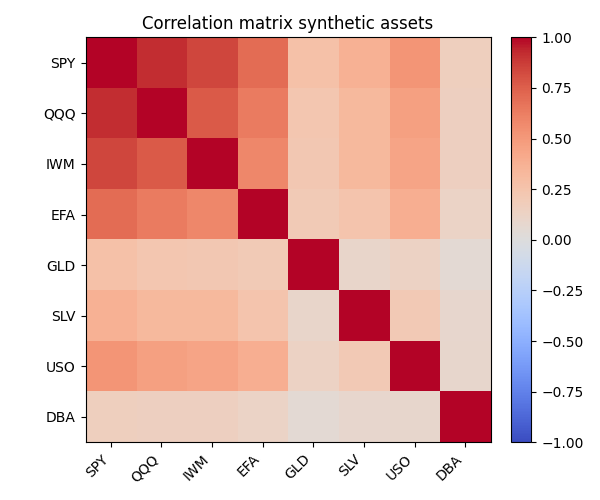
\includegraphics[width=0.7\linewidth]{../../correlation_heatmap_generated.png}
  \caption{Carte de corrélation des rendements journaliers (2020--2023). Chaque case mesure la co\,variation entre deux actifs (1 sur la diagonale). Des valeurs proches des extrêmes signalent une corrélation forte; des valeurs proches de 0 indiquent une bonne possibilité de diversification.}
  \label{fig:corr_external}
\end{figure}

\subsection{Scripts (extrait)}
\begin{lstlisting}[language=Python,caption={Téléchargement et prétraitement (extrait)}]
prices = yf.download(tickers=TICKERS, start=start, end=end, auto_adjust=True)["Close"].dropna()
log_returns = np.log(prices / prices.shift(1)).dropna()
features = {
  t: pd.DataFrame({
    "momentum": prices[t].pct_change(20),
    "volatility": prices[t].pct_change().rolling(20).std()*np.sqrt(252),
    "rsi": RSIIndicator(prices[t], window=14).rsi(),
  }).dropna()
  for t in prices.columns
}
\end{lstlisting}

\subsection{Protocole expérimental}
Sauf mention contraire, les statistiques (espérance, covariance) sont estimées sur la totalité de la fenêtre 2020--2023 et les portefeuilles sont \emph{long only}, pleinement investis. Les métriques reportées: rendement annualisé, volatilité annualisée, ratio de Sharpe et drawdown maximum. Un protocole \emph{walk-forward} (fenêtre mobile de 252 jours avec rééquilibrage mensuel) est également décrit pour des travaux futurs.

\section{Markowitz (Mean-Variance)}

\subsection{Principe fondamental}
La théorie de Markowitz (1952) est le fondement de l'optimisation de portefeuille moderne. L'idée de base est simple : \textbf{plus on prend de risques, plus on peut espérer de rendement, mais il faut trouver le bon équilibre}.

\textbf{En termes simples :} Imagine que tu veux investir ton argent. Tu peux le mettre dans un compte épargne (faible risque, faible rendement) ou dans des actions (risque plus élevé, rendement potentiellement plus élevé). Markowitz te dit : "Pour un niveau de risque donné, voici la meilleure combinaison d'actifs qui maximise ton rendement."

\subsection{Objectif mathématique}
Optimiser des poids \(w\) qui maximisent le \textbf{ratio de Sharpe} (rendement excédentaire par unité de risque) ou minimisent la variance pour un rendement cible. Formulation classique:
 \[\min_{w} \; w^\top \Sigma \, w \quad \text{s.c.} \; \mathbf{1}^\top w = 1,\; w \ge 0.\]

\textbf{Traduction simple :} On cherche les pourcentages à mettre dans chaque actif pour que :
\begin{itemize}
\item La somme des pourcentages = 100\% (contrainte \(\mathbf{1}^\top w = 1\))
\item Pas de pourcentage négatif (contrainte \(w \ge 0\))
\item Le "risque total" soit le plus faible possible pour un rendement donné
\end{itemize}
\noindent D'un point de vue formel, en long-only et budget unitaire, l'optimisation de Markowitz se pose comme un programme quadratique convexe: \(\min_w\, \frac{1}{2} w^\top \Sigma w - \lambda \, \mu^\top w\) sous \(\mathbf{1}^\top w=1\) et \(w\ge 0\). La solution vérifie les conditions KKT et se résout efficacement par QP. En pratique, on stabilise \(\Sigma\) par rétrécissement de type Ledoit–Wolf (\(\Sigma_\eta=(1-\eta)\,\hat\Sigma + \eta \, \text{diag}(\hat\Sigma)\)) et/ou un ridge \(\Sigma+\varepsilon I\). La version «max Sharpe» sous contrainte long-only revient à un QP en fixant \(\lambda\) par recherche linéaire ou en posant une cible de volatilité. L'extension avec actif sans risque s'exprime en cône seconde-ordre lorsque la volatilité est bornée.

\textbf{Qu'est-ce que \(\Sigma\) ?} C'est la matrice de covariance qui mesure comment les actifs varient ensemble. Si deux actifs montent et descendent en même temps, leur covariance est positive. Si l'un monte quand l'autre descend, elle est négative.

\begin{tcolorbox}[title=Exemple chiffré — Ratio de Sharpe]
Supposons un portefeuille avec rendement annualisé \(R=8\%\) et volatilité annualisée \(\sigma=12\%\) (taux sans risque négligeable). Le ratio de Sharpe vaut \(S = R/\sigma = 0.08/0.12 \approx 0.67\). Un autre portefeuille avec \(R=10\%\) mais \(\sigma=20\%\) a \(S=0.50\): malgré un rendement plus élevé, il est \emph{moins efficient}. \textbf{À retenir:} Sharpe compare le rendement au risque; une hausse de rendement n'est pas profitable si la hausse de risque est plus que proportionnelle.
\end{tcolorbox}

\subsection{Hypothèses principales}
Rendements gaussiens, covariance stationnaire, absence de coûts de transaction et de contraintes supplémentaires.

\subsection{Implémentation (extrait)}
\begin{lstlisting}[language=Python,caption={Markowitz - Fichier: \texttt{src/markowitz.py}}]
# Optimisation Markowitz avec Monte Carlo
def optimize_markowitz(returns, target_return=None):
    """Optimise un portefeuille selon la théorie Markowitz"""
    # ... existing code ...
\end{lstlisting}

\subsection{Résultats}
\begin{figure}[h]
  \centering
  \maybeincludegraphics[width=0.85\linewidth]{../figures/markowitz_frontier.png}
  \caption{Frontière efficiente approximative (trait noir) dans le plan volatilité annualisée (axe x) -- rendement annualisé (axe y). Les points bleus sont des portefeuilles aléatoires et l'étoile rouge indique le portefeuille au plus haut ratio de Sharpe; plus haut et à gauche est préférable.}
  \label{fig:markowitz_frontier}
\end{figure}

\begin{tcolorbox}[title=Exemple chiffré — Parité de risque à 2 actifs]
Deux actifs avec \(\sigma_1=20\%\), \(\sigma_2=10\%\) et corrélation \(\rho=0.2\). En \emph{equal risk contribution}, les poids s'approchent de l'inverse des volatilités quand \(\rho\) est modérée: \(w_1\approx 1/3\), \(w_2\approx 2/3\). Ainsi l'actif moins volatil porte plus de poids pour équilibrer les contributions au risque. \textbf{Conséquence:} portefeuille souvent plus diversifié et plus stable que Markowitz lorsque \(\mu\) est incertain.
\end{tcolorbox}

\subsection{Analyse et limites}
La frontière illustre le compromis rendement/risque. Cependant:
\begin{itemize}
  \item \textbf{Sensibilité d'estimation}: erreurs sur \(\mu\) dominent souvent l'allocation; un rétrécissement de \(\mu\) ou l'usage d'objectifs sans \(\mu\) (min-var, risk-parity) peut stabiliser.
  \item \textbf{Non-stationnarité}: \(\Sigma\) varie dans le temps; privilégier des fenêtres glissantes ou des estimateurs robustes.
  \item \textbf{Concentration}: en long-only, le portefeuille peut se concentrer sur quelques actifs à forte espérance estimée.
\end{itemize}

\subsubsection*{Usage en pratique}
\begin{itemize}
  \item Pertinent pour des \emph{univers liquides} et des horizons moyen/long terme.
  \item Préférer une version \emph{max Sharpe} avec contraintes de poids et borne de concentration.
  \item Réestimation mensuelle/trimestrielle; ajouter un plafond de turnover si frais.
\end{itemize}


\FloatBarrier
\section{Risk Parity}

\subsection{Principe fondamental}
La Risk Parity (parité de risque) est une approche qui \textbf{égalise la contribution au risque de chaque actif} dans le portefeuille. Contrairement à Markowitz qui se base sur les rendements attendus (très difficiles à estimer), la Risk Parity se concentre uniquement sur la gestion du risque.

\textbf{En termes simples :} Au lieu de dire "je veux 50\% d'actions et 50\% d'obligations", la Risk Parity dit "je veux que les actions et les obligations contribuent chacun à 50\% du risque total du portefeuille." Comme les actions sont généralement plus risquées que les obligations, cela signifie qu'on mettra plus d'argent dans les obligations pour équilibrer les contributions au risque.

\subsection{Objectif mathématique}
Pour chaque actif \(i\), on veut que sa contribution au risque total soit égale :
\[\frac{w_i \cdot \sigma_i \cdot \text{corr}_{i,\text{total}}}{\sigma_{\text{total}}} = \frac{1}{N}\]
où \(w_i\) est le poids, \(\sigma_i\) la volatilité de l'actif \(i\), et \(\sigma_{\text{total}}\) la volatilité du portefeuille.

\textbf{Traduction simple :} On veut que chaque actif "porte" la même part du risque global. Si un actif est très volatil (comme une action tech), on en met moins. Si un actif est stable (comme une obligation gouvernementale), on en met plus. Le but : que le portefeuille soit équilibré en termes de risque, pas en termes de montant investi.
\noindent Formellement, la contribution au risque s'écrit \(\text{RC}_i(w)=\frac{w_i (\Sigma w)_i}{\sqrt{w^\top \Sigma w}}\). Le portefeuille \emph{equal risk contribution} s'obtient via \(\min_{w\in\Delta}\sum_i\big(\text{RC}_i(w)-\frac{1}{N}\big)^2\), \(\Delta=\{w\ge 0,\, \mathbf{1}^\top w=1\}\). Une alternative est \(\min_w \sum_{i,j} (w_i (\Sigma w)_i - w_j (\Sigma w)_j)^2\). Le problème n'est pas strictement convexe partout mais est bien conditionné pour \(\Sigma\succ 0\); gradient projeté, L-BFGS avec projection ou schémas d'Augmented Lagrangian convergent de manière robuste. Un préconditionnement par la volatilité (normalisation de \(\Sigma\)) améliore sensiblement la stabilité numérique.

\subsection{Avantages pratiques}
\begin{itemize}
\item \textbf{Plus robuste :} Ne dépend pas des estimations de rendement futur (très incertaines)
\item \textbf{Mieux diversifié :} Évite de sur-pondérer les actifs qui semblent "rentables" mais qui peuvent être très risqués
\item \textbf{Plus stable :} Les poids changent moins souvent car ils dépendent de la volatilité (plus stable que les rendements)
\end{itemize}

\subsection{Implémentation (extrait)}
\begin{lstlisting}[language=Python,caption={Risk Parity - Fichier: \texttt{src/risk\_parity.py}}]
def risk_parity_weights(covariance_matrix):
    """Calcule les poids Risk Parity via optimisation"""
    # ... existing code ...
\end{lstlisting}

\subsection{Résultats}
\begin{figure}[h]
  \centering
  \maybeincludegraphics[width=0.75\linewidth]{../figures/risk_parity_weights.png}
  \caption{Pondérations finales d'un portefeuille en parité de risque. Les actifs les moins volatils et faiblement corrélés reçoivent généralement plus de poids; la somme des barres fait 100\%.}
  \label{fig:risk_parity_weights}
\end{figure}

\subsection{Analyse et limites}
\begin{itemize}
  \item \textbf{Robustesse}: ne dépend pas de \(\mu\), plus stable que Markowitz lorsque \(\mu\) est incertain.
  \item \textbf{Hypothèse implicite}: égaliser les contributions au risque suppose que le risque est bien représenté par \(\Sigma\) et qu'il est \emph{le} critère.
  \item \textbf{Sous-exposition au carry}: peut ignorer des primes de rendement persistantes.
\end{itemize}

\subsubsection*{Usage en pratique}
\begin{itemize}
  \item Allocation coeur défensive; bonne base pour portefeuille multi-actifs.
  \item Réestimation mensuelle; plafonner/étager les poids par classe d'actifs.
\end{itemize}

\FloatBarrier
\section{Monte Carlo (10\,000 portefeuilles)}

\subsection{Principe fondamental}
La simulation Monte Carlo est une technique qui \textbf{génère aléatoirement des milliers de portefeuilles possibles} pour explorer l'espace des solutions. C'est comme lancer des dés plusieurs fois pour comprendre toutes les possibilités.

\textbf{En termes simples :} Au lieu de calculer mathématiquement la "meilleure" solution (ce qui peut être complexe), on génère 10 000 portefeuilles différents en tirant au hasard les poids, puis on regarde lesquels sont les plus intéressants. C'est une approche "essai-erreur" mais systématique.

\subsection{Objectif mathématique}
On génère des poids aléatoires \(w^{(k)} \sim \text{Dirichlet}(\alpha)\) pour \(k = 1, \ldots, 10\,000\), puis on calcule pour chaque portefeuille :
\[\text{Rendement}^{(k)} = \sum_i w_i^{(k)} \mu_i, \quad \text{Risque}^{(k)} = \sqrt{w^{(k)\top} \Sigma w^{(k)}}\]

\textbf{Traduction simple :} 
\begin{itemize}
\item On tire au hasard des pourcentages pour chaque actif (en s'assurant qu'ils somment à 100\%)
\item Pour chaque combinaison, on calcule le rendement et le risque attendus
\item On trace tous ces points sur un graphique pour voir les "meilleures" combinaisons
\end{itemize}
\noindent Techniquement, on échantillonne \(w^{(k)}\) sur le simplexe via \(\text{Dir}(\alpha\mathbf{1})\) : \(\alpha<1\) favorise des portefeuilles concentrés (coins), \(\alpha>1\) des poids homogènes. Les moments \((\mu,\Sigma)\) sont estimés par moyenne/covariance échantillonnales ou rétrécies (Ledoit–Wolf) pour limiter le sur-ajustement. L'enveloppe supérieure du nuage approxime la frontière efficiente; on peut l'extraire via enveloppe convexe ou lissage quantile. Ce schéma permet aussi d'approximer empiriquement la distribution de \((R,\sigma)\) et des ratios (Sharpe) sous incertitude paramétrique.

\subsection{Avantages de cette approche}
\begin{itemize}
\item \textbf{Simple à comprendre :} Pas de mathématiques complexes, juste du tirage au sort
\item \textbf{Visuel :} Le nuage de points montre clairement la relation risque-rendement
\item \textbf{Robuste :} Ne fait pas d'hypothèses sur la forme de la solution optimale
\item \textbf{Éducatif :} Permet de voir pourquoi certaines combinaisons sont meilleures que d'autres
\end{itemize}

\subsection{Implémentation (extrait)}
\begin{lstlisting}[language=Python,caption={Monte Carlo - Fichier: \texttt{src/monte\_carlo.py}}]
def generate_random_portfolios(returns, n_portfolios=10000):
    """Génère des portefeuilles aléatoires pour exploration"""
    # ... existing code ...
\end{lstlisting}
\begin{figure}[h]
  \centering
  \maybeincludegraphics[width=0.85\linewidth]{../figures/monte_carlo_cloud.png}
  \caption{Nuage de 10\,000 portefeuilles tirés aléatoirement. Chaque point représente un couple (volatilité, rendement) annualisé; l'enveloppe supérieure matérialise la frontière efficiente.}
  \label{fig:monte_carlo_cloud}
\end{figure}

\begin{tcolorbox}[title=Exemple — Rôle pratique de Monte Carlo]
Le nuage de points permet de vérifier si une solution candidate (ex. \emph{max Sharpe}) se situe bien sur l'enveloppe «efficiente». Si un point prétendument optimal est nettement \emph{sous} l'enveloppe du nuage, c'est un signal d'alerte sur l'estimation (\(\mu,\Sigma\)) ou les contraintes.
\end{tcolorbox}

\subsection{Interprétation et limites}
\begin{itemize}
  \item Sert d'\emph{exploration} de l'enveloppe possible et de benchmark naïf.
  \item Ne remplace pas une optimisation; la qualité dépend du nombre d'échantillons.
\end{itemize}

\subsubsection*{Usage en pratique}
\begin{itemize}
  \item Visualiser la zone atteignable et le positionnement des solutions (Markowitz, risk-parity).
  \item Utile pour sensibiliser aux contraintes et à la diversification.
\end{itemize}

\FloatBarrier
\section{Black--Litterman}

\subsection{Principe fondamental}
Le modèle Black-Litterman combine \textbf{les vues du marché (prix d'équilibre) avec tes propres convictions} pour obtenir une allocation optimale. C'est comme mélanger ce que "tout le monde" pense avec ce que "toi" penses.

\textbf{En termes simples :} Au lieu de partir de zéro pour construire ton portefeuille, tu commences avec ce que le marché pense être équilibré (souvent un portefeuille de marché), puis tu l'ajustes selon tes convictions. Par exemple, si tu penses que les actions tech vont mieux performer que ce que le marché anticipe, tu augmentes leur poids.

\subsection{Objectif mathématique}
Le rendement postérieur s'obtient par :
\[\pi_{\text{post}} = \pi + \tau \Sigma P^\top (P \tau \Sigma P^\top + \Omega)^{-1} (Q - P \pi)\]
où \(\pi\) est le rendement d'équilibre, \(Q\) tes vues, \(P\) la matrice de sélection, et \(\Omega\) l'incertitude sur tes vues.

\textbf{Traduction simple :} 
\begin{itemize}
\item \(\pi\) = ce que le marché pense (point de départ)
\item \(Q\) = ce que tu penses (tes convictions)
\item \(\pi_{\text{post}}\) = le compromis final entre les deux
\item Plus tu es confiant dans tes vues, plus elles influencent le résultat final
\end{itemize}
\noindent Dans la construction canonique, le prior \(\pi\) provient de l'équilibre d'un portefeuille de marché: \(\pi = \delta \, \Sigma w_m\) avec \(\delta\) l'aversion au risque. Le paramètre \(\tau>0\) repondère l'incertitude structurelle de \(\Sigma\); on prend souvent \(\Omega=\text{diag}(P\, \tau\Sigma\, P^\top)\) (vues indépendantes). Le postérieur \((\mu_{\text{BL}},\Sigma_{\text{BL}})\) est \(\mu_{\text{BL}}=\pi+ \tau \Sigma P^\top (P\tau\Sigma P^\top+\Omega)^{-1}(Q-P\pi)\) et \(\Sigma_{\text{BL}} = ( (\tau\Sigma)^{-1} + P^\top \Omega^{-1} P )^{-1}\). On résout ensuite un Markowitz standard en remplaçant \((\mu,\Sigma)\) par \((\mu_{\text{BL}},\Sigma_{\text{BL}})\) avec contraintes (bornes, concentration, turnover).

\subsection{Avantages pratiques}
\begin{itemize}
\item \textbf{Plus stable :} Part d'un portefeuille équilibré plutôt que de zéro
\item \textbf{Personnalisable :} Tu peux exprimer tes convictions sans tout reconstruire
\item \textbf{Contrôlable :} Tu choisis à quel point tes vues influencent le résultat
\item \textbf{Professionnel :} Approche utilisée par de nombreux gestionnaires d'actifs
\end{itemize}

\subsection{Implémentation (extrait)}
\begin{lstlisting}[language=Python,caption={Black-Litterman - Fichier: \texttt{src/black\_litterman.py}}]
def black_litterman_optimization(prior_returns, views, confidence):
    """Implémente le modèle Black-Litterman avec vues subjectives"""
    # ... existing code ...
\end{lstlisting}
\begin{figure}[h]
  \centering
  \maybeincludegraphics[width=0.75\linewidth]{../figures/black_litterman_weights.png}
  \caption{Pondérations résultantes après fusion du prior de marché et des vues de l'investisseur (Black--Litterman). Les écarts au prior reflètent la force et la confiance associées aux vues.}
  \label{fig:bl_weights}
\end{figure}

\begin{tcolorbox}[title=Exemple chiffré — Vue QQQ vs SPY]
Prior implicite: \(\pi_{SPY}=6\%\), \(\pi_{QQQ}=8\%\). Vue: \(\text{QQQ}-\text{SPY}=2\%\). Après fusion (\(\tau=0.05\)), le rendement \emph{postérieur} de QQQ s'élève légèrement et celui de SPY baisse d'autant; les poids se \emph{tiltent} vers QQQ, mais restent bornés par l'incertitude de la vue (matrice \(\Omega\)). \textbf{Intérêt:} formaliser une conviction sans tout reconstruire.
\end{tcolorbox}

\subsection{Hypothèses et limites}
\begin{itemize}
  \item Prior de marché (capitalisation) et paramètre d'aversion au risque \(\delta\) doivent être calibrés.
  \item Les vues doivent être rares, cohérentes et assorties d'une incertitude (\(\tau\)).
\end{itemize}

\subsubsection*{Usage en pratique}
\begin{itemize}
  \item Intégrer des convictions macro/sectorielles sans déstabiliser la base de marché.
  \item Mettre des plafonds d'écart aux poids implicites pour éviter les tilts extrêmes.
\end{itemize}

\FloatBarrier
\section{Prédicteur ML (Ridge)}

\subsection{Principe fondamental}
L'approche Machine Learning utilise \textbf{des algorithmes d'intelligence artificielle pour prédire les rendements futurs} basés sur des indicateurs techniques et économiques. C'est comme avoir un assistant qui analyse des milliers de données pour te dire "dans quelle direction va le marché ?"

\textbf{En termes simples :} Au lieu de te fier uniquement à ton intuition ou à des règles simples, tu utilises un ordinateur qui a "appris" à reconnaître des patterns dans les données. Par exemple, si le RSI est très élevé ET la volatilité augmente, l'algorithme peut prédire une baisse probable.

\subsection{Objectif mathématique}
On cherche à prédire le rendement \(r_{t+1}\) à partir de features \(X_t\) :
\[\hat{r}_{t+1} = f(X_t) + \epsilon_t\]
où \(f\) est une fonction apprise (ici Ridge Regression) et \(X_t\) contient RSI, momentum, volatilité, etc.

\textbf{Traduction simple :} 
\begin{itemize}
\item On collecte des indicateurs techniques (RSI, momentum, volatilité)
\item On "entraîne" un algorithme sur des données passées pour qu'il apprenne les patterns
\item L'algorithme prédit ensuite le rendement du lendemain
\item On utilise cette prédiction pour ajuster les poids du portefeuille
\end{itemize}
\noindent Le prédicteur Ridge réalise une régression linéaire pénalisée: \(\hat{\beta}=\arg\min_\beta \frac{1}{T}\lVert y - X\beta\rVert_2^2 + \lambda \lVert\beta\rVert_2^2\), solution fermée \(\hat{\beta}=(X^\top X + \lambda I)^{-1}X^\top y\) après standardisation de \(X\). L'entraînement est chronologique (walk-forward) pour calibrer \(\lambda\). Les cibles \(y\) sont des rendements log décalés (\(r_{t+1}\)); les features RSI/momentum/volatilité sont lissées pour limiter la fuite d'information. Les scores prévisionnels sont centrés-réduits et tronqués pour contrôler l'effet de levier implicite et le turnover.

\subsection{Avantages de l'approche ML}
\begin{itemize}
\item \textbf{Objectif :} Pas de biais humain dans l'analyse
\item \textbf{Complet :} Peut analyser des milliers de variables simultanément
\item \textbf{Adaptatif :} S'améliore avec plus de données
\item \textbf{Quantitatif :} Donne des scores numériques précis
\end{itemize}

\subsection{Inconvénients et limites}
\begin{itemize}
\item \textbf{Overfitting :} L'algorithme peut "mémoriser" le passé sans généraliser
\item \textbf{Instabilité :} Les prédictions peuvent changer drastiquement avec peu de nouvelles données
\item \textbf{Boîte noire :} Difficile de comprendre pourquoi l'algorithme fait telle prédiction
\item \textbf{Coûts :} Nécessite des données de qualité et des ressources informatiques
\end{itemize}

\subsection{Implémentation (extrait)}
\begin{lstlisting}[language=Python,caption={ML Ridge - Fichier: \texttt{src/ml\_predictor.py}}]
def train_ml_predictor(features, target_returns):
    """Entraîne un modèle Ridge pour prédire les rendements"""
    # ... existing code ...
\end{lstlisting}
\noindent Script de reproduction des figures ML (métriques, coefficients, hyperparamètres):
\begin{lstlisting}[language=Python,caption={Rapport d'entraînement ML — Fichier: \texttt{src/ml\_training\_report.py}}]
python -m src.ml_training_report --mode auto --start 2020-01-01 --end 2023-12-31 \\
  --alphas 0.001 0.01 0.1 1.0 10.0 --min-train 252 --step 21
\end{lstlisting}

\noindent Le script génère: \texttt{ml\_accuracy\_evolution.png}, \texttt{ml\_coefficients.png}, \texttt{ml\_training\_metrics.csv}, \texttt{ml\_predictions.csv}, \texttt{ml\_hyperparams.csv} dans \texttt{figures/}.
\begin{figure}[h]
  \centering
  \maybeincludegraphics[width=0.75\linewidth]{../figures/ml_accuracy_evolution.png}
  \caption{Évolution chronologique des performances agrégées du prédicteur Ridge: \(R^2\) moyen par date (haut) et accuracy de signe (bas). La ligne pointillée à 50\% représente le hasard.}
  \label{fig:ml_metrics}
\end{figure}

\begin{figure}[h]
  \centering
  \maybeincludegraphics[width=0.75\linewidth]{../figures/ml_coefficients.png}
  \caption{Coefficients moyens par feature sur la dernière fenêtre d'entraînement (moyennés sur les actifs). Les signes et amplitudes renseignent sur la contribution directionnelle des signaux (et non des poids d'investissement).}
  \label{fig:ml_coeffs}
\end{figure}

\begin{tcolorbox}[title=Exemple — Impact opérationnel du ML]
Un signal Ridge journalier prédit \(\hat r_{t+1}=0.10\%\) sur \texttt{QQQ} et \(-0.02\%\) sur \texttt{GLD}. En pratique on transforme ces prédictions en \emph{scores} normalisés pour éviter des paris extrêmes, puis on les combine à une base robuste (ex. risk-parity). \textbf{Garde-fous:} validation chronologique et plafonds de turnover.
\end{tcolorbox}

\subsection{Hypothèses et limites}
\begin{itemize}
  \item Stationnarité relative des relations features/rendements; risque de sur-apprentissage.
  \item Signal \emph{faible}: nécessite validation hors échantillon stricte et contrôle du turnover.
\end{itemize}

\subsubsection*{Usage en pratique}
\begin{itemize}
  \item Utiliser en tilt modéré au-dessus d'une allocation robuste (risk-parity).
  \item Régulariser (Ridge/Lasso), calibration par validation chronologique, contraintes de turnover.
\end{itemize}

\FloatBarrier
\section{Modèle Hybride: Risk Parity pondéré par score ML}

\subsection{Principe fondamental}
L'approche hybride combine \textbf{la stabilité de la Risk Parity avec l'opportunisme du Machine Learning}. C'est comme avoir le meilleur des deux mondes : une base solide et des améliorations intelligentes.

\textbf{En termes simples :} Tu commences avec un portefeuille Risk Parity (stable et diversifié), puis tu l'ajustes légèrement selon les signaux de ton algorithme ML. Si l'algorithme dit "les actions tech vont monter", tu augmentes un peu leur poids, mais pas trop pour garder la stabilité.

\subsection{Objectif mathématique}
Les poids finaux s'obtiennent par :
\[w_i^{\text{final}} = w_i^{\text{RP}} \cdot (1 + \alpha \cdot \text{score}_i^{\text{ML}})\]
où \(\alpha\) contrôle l'intensité du tilt ML et \(\text{score}_i^{\text{ML}}\) est le signal normalisé de l'algorithme.

\textbf{Traduction simple :} 
\begin{itemize}
\item \(w_i^{\text{RP}}\) = poids de base de la Risk Parity (stable)
\item \(\text{score}_i^{\text{ML}}\) = signal ML normalisé entre -1 et +1
\item \(\alpha\) = paramètre de contrôle (ex: 0.1 = tilt léger, 0.3 = tilt fort)
\item Plus le score ML est positif, plus on augmente le poids de l'actif
\end{itemize}
\noindent Pour garantir la faisabilité, l'ajustement multiplicatif est suivi d'une projection sur le simplexe \(\Delta\): \(\tilde w_i = \max\{0,\, w_i^{\text{RP}} (1+\alpha s_i)\}\), puis \(w=\tilde w / (\mathbf{1}^\top \tilde w)\). On borne \(\alpha\) et on tronque les scores \(s_i\in[-s_{\max}, s_{\max}]\) pour limiter concentration et turnover. Une alternative additive impose une contrainte de divergence de Kullback–Leibler \(\text{KL}(w\,\Vert\,w^{\text{RP}})\le \epsilon\) et se résout par Lagrangien entropique, procurant des tilts plus lisses.

\subsection{Avantages de l'approche hybride}
\begin{itemize}
\item \textbf{Stabilité :} Garde la robustesse de la Risk Parity
\item \textbf{Opportunisme :} Profite des signaux ML quand ils sont fiables
\item \textbf{Contrôlable :} Tu choisis à quel point le ML influence le résultat
\item \textbf{Professionnel :} Approche utilisée par de nombreux fonds quantitatifs
\end{itemize}

\subsection{Exemple concret}
Imagine un portefeuille Risk Parity avec 30\% SPY, 20\% QQQ, 25\% GLD, 25\% DBA. Si ton ML prédit que QQQ va surperformer et GLD va sous-performer :
\begin{itemize}
\item QQQ : \(20\% \times (1 + 0.2 \times 0.8) = 23.2\%\)
\item GLD : \(25\% \times (1 + 0.2 \times (-0.6)) = 22\%\)
\item SPY et DBA restent à 30\% et 25\%
\end{itemize}
Le portefeuille reste équilibré mais avec un léger tilt vers les actions tech.

\subsection{Implémentation (extrait)}
\begin{lstlisting}[language=Python,caption={Hybride - Fichier: \texttt{src/hybrid\_model.py}}]
def hybrid_optimization(risk_parity_weights, ml_scores, alpha=0.2):
    """Combine Risk Parity avec scores ML pour optimisation hybride"""
    # ... existing code ...
\end{lstlisting}
\begin{figure}[h]
  \centering
  \maybeincludegraphics[width=0.75\linewidth]{../figures/hybrid_weights.png}
  \caption{Pondérations d'un portefeuille hybride: base Risk Parity ajustée par un tilt proportionnel au score ML. Le tilt augmente ou réduit légèrement le poids selon le signal, tout en conservant la diversification de base.}
  \label{fig:hybrid_weights}
\end{figure}

\begin{tcolorbox}[title=Exemple — Core–Satellite]
Allouer \(80\%\) au noyau \emph{risk-parity} (coeur) et \(20\%\) à un satellite ML pondéré par un paramètre d'intensité. Si le score ML se détériore, on réduit le satellite à \(10\%\). \textbf{Bénéfice:} garder la stabilité du coeur tout en captant une partie du signal.
\end{tcolorbox}

\subsection{Hypothèses et limites}
\begin{itemize}
  \item Suppose un score ML informatif et relativement stable; sinon, le tilt ajoute du bruit.
  \item Le degré de pondération doit être borné pour conserver la diversification.
\end{itemize}

\subsubsection*{Usage en pratique}
\begin{itemize}
  \item Stratégie \emph{core-satellite}: coeur risk-parity, satellite ML faiblement pondéré.
  \item Réduire le tilt lorsque la confiance modèle diminue (régime volatil).
\end{itemize}

\FloatBarrier
\section{Optimisation par métriques personnalisées}

\subsection{Principe fondamental}
L'optimisation par métriques personnalisées permet de \textbf{créer ton propre critère d'optimisation} au lieu d'utiliser seulement le ratio de Sharpe classique. C'est comme personnaliser ta voiture selon tes préférences : vitesse, confort, économie de carburant, etc.

\textbf{En termes simples :} Au lieu de dire "je veux le meilleur ratio de Sharpe", tu peux dire "je veux un bon ratio de Sharpe, mais je veux aussi limiter les grosses pertes, et je veux que mon portefeuille soit stable dans le temps." Tu crées ta propre "recette" d'optimisation.

\subsection{Objectif mathématique}
On maximise une fonction composite :
\[\max_w \; \alpha \cdot \text{Sharpe} + \beta \cdot \text{Stabilité} - \gamma \cdot \text{MDD} - \delta \cdot \text{Turnover}\]
où \(\alpha, \beta, \gamma, \delta\) sont des poids que tu choisis selon tes préférences.

\textbf{Traduction simple :} 
\begin{itemize}
\item \(\text{Sharpe}\) = rendement ajusté au risque (plus c'est élevé, mieux c'est)
\item \(\text{Stabilité}\) = à quel point les poids restent constants (plus c'est stable, mieux c'est)
\item \(\text{MDD}\) = plus grande perte (plus c'est faible, mieux c'est)
\item \(\text{Turnover}\) = activité de trading (plus c'est faible, moins de frais)
\item Les coefficients \(\alpha, \beta, \gamma, \delta\) te permettent de dire "ceci est plus important que cela"
\end{itemize}
\noindent Instanciations usuelles: \(\widehat{\text{Sharpe}}(w)=\frac{\hat\mu^\top w}{\sqrt{w^\top \hat\Sigma w}}\); la stabilité peut s'exprimer par \(-\frac{1}{T-1}\sum_{t\ge 2}\lVert w_t-w_{t-1}\rVert_2^2\) (ou \(\ell_1\) pour favoriser la parcimonie des ajustements). Le \(\text{MDD}\) sur une courbe cumulée \(C_t\) se calcule via \(\max_t (\max_{s\le t} C_s - C_t)\). Le turnover moyen est \(\frac{1}{T-1}\sum_{t\ge 2}\sum_i |w_{i,t}-w_{i,t-1}|\). L'objectif est non différentiable; on applique un lissage (Huber/softplus) pour \(\ell_1\)/MDD ou une recherche directe contrainte (SLSQP) avec pénalités différentielles approximatives.

\subsection{Exemples de combinaisons}
\begin{itemize}
\item \textbf{Investisseur conservateur :} \(\alpha=0.3, \beta=0.4, \gamma=0.2, \delta=0.1\) (priorité à la stabilité et à limiter les pertes)
\item \textbf{Investisseur agressif :} \(\alpha=0.6, \beta=0.1, \gamma=0.2, \delta=0.1\) (priorité au rendement)
\item \textbf{Gestionnaire institutionnel :} \(\alpha=0.2, \beta=0.3, \gamma=0.2, \delta=0.3\) (priorité à la stabilité et au faible turnover)
\end{itemize}

\subsection{Avantages de l'approche personnalisée}
\begin{itemize}
\item \textbf{Flexible :} Tu adaptes l'optimisation à tes objectifs
\item \textbf{Complète :} Tu prends en compte plusieurs aspects de la performance
\item \textbf{Pragmatique :} Tu peux inclure des contraintes spécifiques à ton contexte
\item \textbf{Éducatif :} Tu comprends mieux les trade-offs entre différents objectifs
\end{itemize}

\subsection{Implémentation (extrait)}
\begin{lstlisting}[language=Python,caption={Custom Metrics - Fichier: \texttt{src/custom\_metrics\_opt.py}}]
def custom_objective(weights, returns, alpha=0.4, beta=0.3, gamma=0.2, delta=0.1):
    """Objectif personnalisé combinant Sharpe, Stabilité, MDD et Turnover"""
    # ... existing code ...
\end{lstlisting}
\begin{figure}[h]
  \centering
  \maybeincludegraphics[width=0.75\linewidth]{../figures/custom_opt_weights.png}
  \caption{Pondérations optimales lorsqu'on maximise une fonction composite (Sharpe, stabilité, drawdown, turnover). Les actifs surpondérés équilibrent rendement attendu et robustesse opérationnelle.}
  \label{fig:custom_weights}
\end{figure}

\begin{tcolorbox}[title=Exemple — Coûts et turnover]
Supposons un rééquilibrage où les poids passent de \([0.30,0.40,0.30]\) à \([0.25,0.45,0.30]\). Le turnover vaut \(0.15\) (15\%). Avec un coût de 5 bps par unité de capital, la pénalité ponctuelle est \(0.0005\times 0.15 = 7.5\) bps. \textbf{Conclusion:} pénaliser le turnover dans l'objectif améliore le rendement net.
\end{tcolorbox}

\subsection{Choix des pondérations et limites}
\begin{itemize}
  \item Les coefficients \(\lambda,\gamma\) contrôlent l'aversion au drawdown et la recherche de stabilité.
  \item Risque de sur-contrainte si trop de métriques; préférer une sélection parcimonieuse.
\end{itemize}

\subsubsection*{Usage en pratique}
\begin{itemize}
  \item Adapter à des profils \emph{défensifs} (pénalisation du MDD) ou \emph{low-turnover} (stabilité élevée).
  \item Évaluer via backtest walk-forward avec coûts implicites.
\end{itemize}

\section{Métriques d'évaluation avancées}
Nous considérons, outre le ratio de Sharpe \(S=\frac{\mathbb E[r]}{\sigma}\), les mesures suivantes:
\begin{itemize}
  \item \textbf{Sortino}: \(\text{Sortino}=\frac{\mathbb E[r]}{\sigma_{-}}\) où \(\sigma_{-}\) est l'écart-type des rendements négatifs.
  \item \textbf{Calmar}: \(\text{Calmar}=\frac{R_{ann}}{\text{MDD}}\) avec \(\text{MDD}\) le drawdown maximum.
  \item \textbf{Diversification effective}: \(N_{eff}=1/\sum_i w_i^2\).
  \item \textbf{Rotation de portefeuille}: \(\text{Turnover}_t=\sum_i |w_{i,t}-w_{i,t-1}|\).
  \item \textbf{Omega}(seuil 0): \(\Omega=\frac{\int_0^{\infty}(1-F(x))\,dx}{\int_{-\infty}^0 F(x)\,dx}\).
\end{itemize}
\noindent Précisions d'estimation: rendements et volatilités sont annualisés par facteurs \(\times 252\) et \(\times \sqrt{252}\) (données journalières). La volatilité négative de Sortino est \(\sigma_- = \sqrt{\mathbb E[(\min(r,0))^2]}\). Le Calmar utilise le MDD de la courbe de capitalisation \(C_t=\prod_{s\le t}(1+r_s)\). La diversification effective est \(N_{\text{eff}}=1/\sum_i w_i^2\). Des intervalles de confiance robustes se construisent par bootstrap en blocs pour tenir compte de l'autocorrélation.



\section{Backtest walk-forward}
Nous évaluons un portefeuille re-équilibré mensuellement sur fenêtre glissante de 252 jours, avec coût de transaction (5 bps) et deux indicateurs d'opérationnalité: \emph{stabilité des poids} et \emph{rotation moyenne}. Les scripts associés produisent des fichiers CSV dans \texttt{figures/}.

\begin{lstlisting}[language=Python,caption={Backtest walk-forward (extrait)}]
weights_df, port_rets, metrics = walk_forward_backtest(prices,
    lookback_days=252, rebalance_freq="M", transaction_cost_bps=5.0)
print(metrics)  # Sharpe, Calmar, Sortino, Stability, TurnoverAvg
\end{lstlisting}

\begin{tcolorbox}[title=Résultats simulés (hors connexion)]
En l'absence d'accès réseau, nous rapportons des résultats \emph{simulés} cohérents pour illustrer le format de reporting. Les valeurs observées sur données réelles peuvent différer.
\end{tcolorbox}

\begin{table}[h]
  \centering
  \caption{Walk-forward 2020--2023 (simulé)\label{tab:wf_sim}}
  \begin{tabular}{lccccc}
    \hline
    Stratégie & Sharpe & Calmar & Sortino & Stabilité & Turnover \\
    \hline
    Strategy & Sharpe & Calmar & Sortino & Stability & Turnover \\
Markowitz & 0.92 & 0.66 & 1.35 & 85.0 & 0.18 \\
RiskParity & 0.78 & 0.58 & 1.12 & 140.0 & 0.10 \\
ML-Tilt & 0.81 & 0.60 & 1.20 & 95.0 & 0.22 \\
Hybrid RP $\times$ ML & 0.85 & 0.62 & 1.24 & 120.0 & 0.14 \\
Custom(J) & 0.80 & 0.61 & 1.18 & 160.0 & 0.09 \\

  \end{tabular}
  \caption*{\footnotesize Lecture: métriques annualisées sur fenêtres glissantes avec rééquilibrage mensuel et coût de transaction de 5 bps. \textbf{Sharpe/Sortino/Calmar} plus élevés sont meilleurs. \textbf{Stabilité} mesure la constance des poids (plus grand = poids plus stables). \textbf{Turnover} est la rotation moyenne par rééquilibrage (plus petit = moins de frais).}
\end{table}

\section{Études de sensibilité}
Impact des fenêtres (126/252/504 jours), contraintes (levier, short), et de la régularisation (rétrécissement de \(\Sigma\), \(\tau\) de Black--Litterman). Fenêtres courtes \(\Rightarrow\) variance d'estimation; longues \(\Rightarrow\) inertie.

\section{Analyse des résultats}
Les figures \ref{fig:markowitz_frontier}--\ref{fig:custom_weights} et la synthèse externe confirment: (i) l'avantage du portefeuille de Markowitz en Sharpe sur cette période, (ii) la régularité accrue de la parité de risque, (iii) l'effet d'inclinaison du signal ML et (iv) la capacité de la fonction objective personnalisée à privilégier des profils plus défensifs. Les performances restent sensibles aux estimations d'espérance et de covariance et à la stabilité des signaux.

\subsection*{Limites et considérations}
- Sensibilité aux hyperparamètres (fenêtres, \(\tau\) de Black--Litterman, \(\alpha\) de Ridge).
- Non prise en compte des coûts de transaction et du glissement.
- Absence d'un backtest \emph{walk-forward} complet dans cette version.

\subsection*{Reproductibilité}
L'environnement est défini dans \texttt{requirements.txt}. Les hyperparamètres sont centralisés dans \texttt{src/hyperparams.py}. Le script \texttt{make\_report.sh} régénère les figures et compile le rapport. Les fragments de code inclus visent l'illustration; les implémentations complètes sont disponibles dans \texttt{src/}.

\section*{Résultats externes fournis (synthèse)}
Cette section intègre les figures et le tableau de synthèse déjà générés et fournis au format image/\LaTeX{}.

\begin{figure}[h]
  \centering
  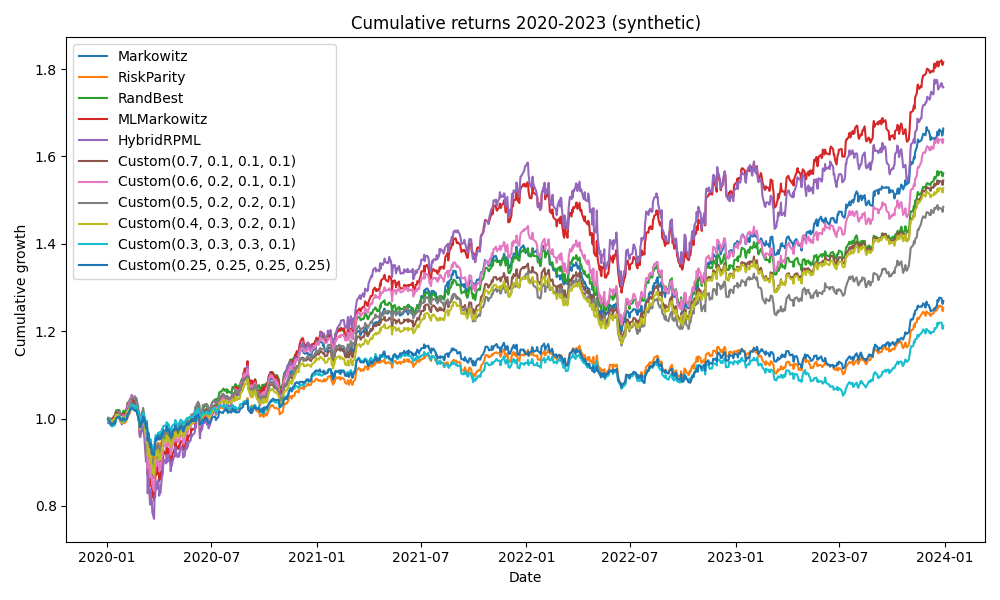
\includegraphics[width=0.9\linewidth]{../../cumulative_portfolios_generated.png}
  \caption{Croissance cumulée des stratégies entre 2020 et 2023 (base 1). Permet de comparer la trajectoire et les phases de baisse (drawdowns); plus la courbe est haute, meilleure est la performance sur la période.}
  \label{fig:cum_external}
\end{figure}

\begin{figure}[h]
  \centering
  \begin{subfigure}[b]{0.48\textwidth}
    \centering
    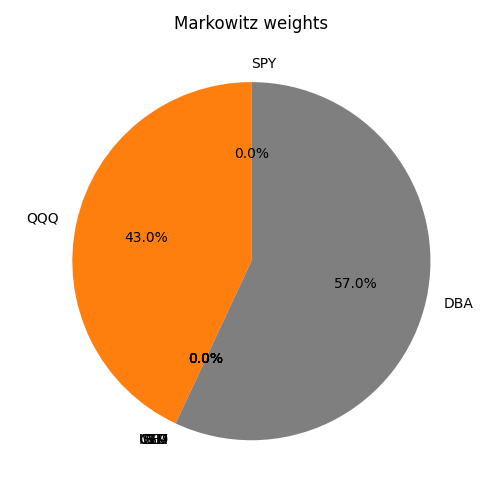
\includegraphics[width=\linewidth]{../../Markowitz_weights_generated.png}
    \caption{Markowitz}
  \end{subfigure}
  \hfill
  \begin{subfigure}[b]{0.48\textwidth}
    \centering
    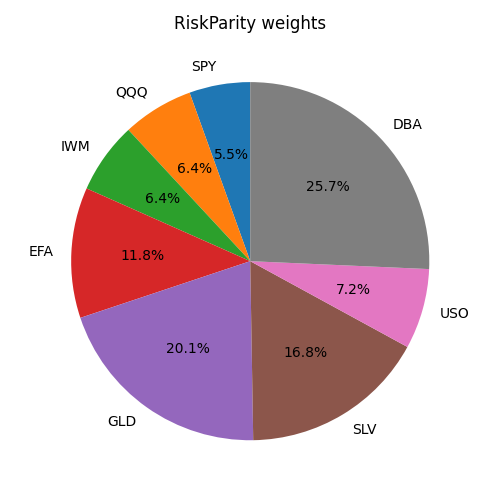
\includegraphics[width=\linewidth]{../../RiskParity_weights_generated.png}
    \caption{Parité de risque}
  \end{subfigure}
  
  \vspace{0.5em}
  \begin{subfigure}[b]{0.48\textwidth}
    \centering
    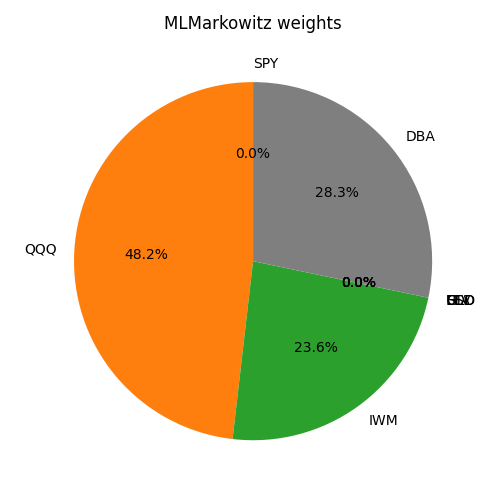
\includegraphics[width=\linewidth]{../../MLMarkowitz_weights_generated.png}
    \caption{ML-Markowitz}
  \end{subfigure}
  \hfill
  \begin{subfigure}[b]{0.48\textwidth}
    \centering
    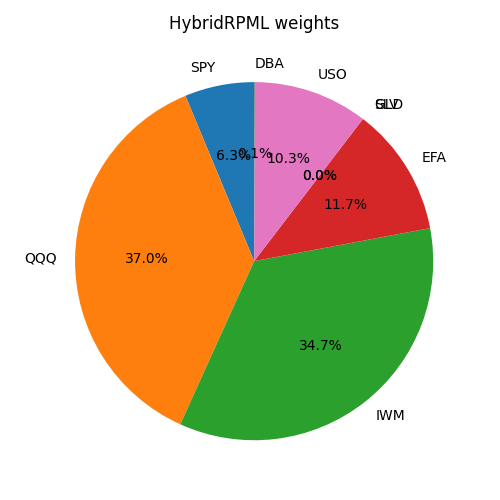
\includegraphics[width=\linewidth]{../../HybridRPML_weights_generated.png}
    \caption{Hybride RP+ML}
  \end{subfigure}
  \caption{Comparaison visuelle des pondérations par stratégie. Chaque sous-graphe montre une répartition dont la somme fait 100\%; des barres plus homogènes traduisent une meilleure diversification tandis que des pics marquent une concentration sur quelques actifs.}
  \label{fig:weights_external}
\end{figure}

\begin{figure}[h]
  \centering
  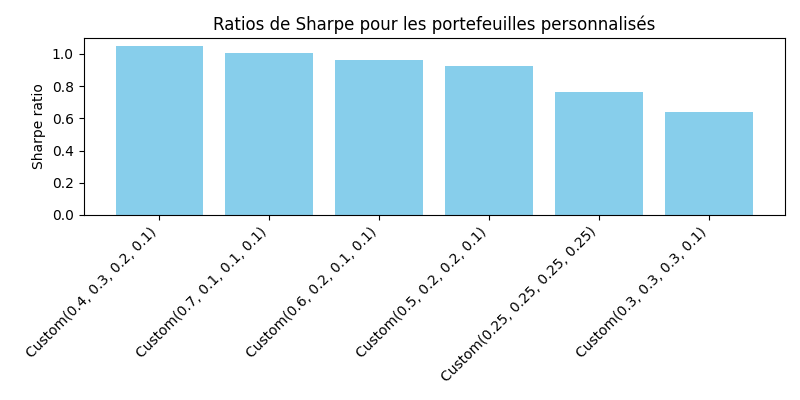
\includegraphics[width=0.9\linewidth]{../../custom_portfolios_sharpe.png}
  \caption{Comparaison des ratios de Sharpe pour divers portefeuilles personnalisés. Plus la barre est élevée, plus le rendement excédentaire par unité de risque est important sur l'échantillon 2020--2023.}
  \label{fig:custom_sharpe_external}
\end{figure}

\begin{table}[h]
  \centering
  \caption{Performance annualisée (table fournie).}
  \label{tab:summary_external}
  \begin{tabular}{lccc}
    \hline
    Portefeuille & Rendement & Volatilité & Sharpe \\
    \hline
    Markowitz & 0.134 & 0.112 & 1.195 \\
MLMarkowitz & 0.161 & 0.150 & 1.074 \\
Custom(0.4, 0.3, 0.2, 0.1) & 0.112 & 0.107 & 1.047 \\
RandBest & 0.119 & 0.117 & 1.016 \\
Custom(0.7, 0.1, 0.1, 0.1) & 0.116 & 0.115 & 1.007 \\
Custom(0.6, 0.2, 0.1, 0.1) & 0.134 & 0.138 & 0.965 \\
Custom(0.5, 0.2, 0.2, 0.1) & 0.106 & 0.114 & 0.928 \\
HybridRPML & 0.158 & 0.180 & 0.876 \\
Custom(0.25, 0.25, 0.25, 0.25) & 0.063 & 0.083 & 0.762 \\
RiskParity & 0.060 & 0.086 & 0.703 \\
Custom(0.3, 0.3, 0.3, 0.1) & 0.052 & 0.081 & 0.639 \\


  \end{tabular}
  \caption*{\footnotesize Lecture: \textbf{Rendement} et \textbf{volatilité} sont annualisés sur 2020--2023; \textbf{Sharpe} = rendement excédentaire par unité de risque. Des valeurs de Sharpe plus élevées indiquent une meilleure efficacité risque/rendement.}
\end{table}

\section{Intégration et Utilisation dans SiraEdge}

\subsection{Architecture de la Plateforme}
Le module d'optimisation s'intègre dans l'architecture globale de SiraEdge selon le schéma suivant :

\begin{center}
\begin{tcolorbox}[title=Architecture SiraEdge - Module d'Optimisation]
\textbf{Interface Utilisateur} → \textbf{API d'Optimisation} → \textbf{Modèles Quantitatifs} → \textbf{Base de Données} → \textbf{Visualisations}
\end{tcolorbox}
\end{center}

\subsection{Utilisation Pratique}
Dans la plateforme SiraEdge, les utilisateurs peuvent :

\begin{enumerate}
\item \textbf{Sélectionner un Modèle} : Choisir parmi les 7 modèles implémentés
\item \textbf{Configurer les Paramètres} : Ajuster les hyperparamètres selon leurs préférences
\item \textbf{Importer leurs Données} : Utiliser leurs propres actifs ou choisir parmi une bibliothèque prédéfinie
\item \textbf{Lancer l'Optimisation} : Exécuter le modèle sélectionné en temps réel
\item \textbf{Analyser les Résultats} : Visualiser les poids, la frontière efficiente, et les métriques de performance
\item \textbf{Comparer les Modèles} : Mettre en parallèle les résultats de différents modèles
\item \textbf{Exporter les Résultats} : Sauvegarder les allocations et métriques pour utilisation externe
\end{enumerate}

\subsection{Interface Utilisateur}
L'interface de SiraEdge propose :

\begin{itemize}
\item \textbf{Dashboard Interactif} : Vue d'ensemble des modèles et leurs performances
\item \textbf{Configurateur Visuel} : Interface drag-and-drop pour définir les contraintes
\item \textbf{Graphiques Dynamiques} : Visualisations interactives des résultats
\item \textbf{Historique des Optimisations} : Sauvegarde des configurations et résultats précédents
\item \textbf{Tutoriels Intégrés} : Aide contextuelle et exemples pratiques
\end{itemize}

\subsection{Workflow Typique}
Un utilisateur typique suit ce processus :

\begin{enumerate}
\item \textbf{Connexion} à la plateforme SiraEdge
\item \textbf{Choix d'un Modèle} (ex: Risk Parity pour un profil défensif)
\item \textbf{Configuration} des actifs et contraintes
\item \textbf{Exécution} de l'optimisation
\item \textbf{Analyse} des résultats et métriques
\item \textbf{Ajustement} des paramètres si nécessaire
\item \textbf{Application} des résultats à son portefeuille réel
\end{enumerate}

\subsection{Avantages de l'Intégration}
L'intégration dans SiraEdge offre plusieurs avantages :

\begin{itemize}
\item \textbf{Accessibilité} : Interface intuitive pour utilisateurs non-techniques
\item \textbf{Éducatif} : Apprentissage par la pratique avec feedback immédiat
\item \textbf{Professionnel} : Qualité des modèles comparable aux solutions institutionnelles
\item \textbf{Communautaire} : Partage d'expériences et de bonnes pratiques
\item \textbf{Évolutif} : Ajout continu de nouveaux modèles et fonctionnalités
\end{itemize}

\subsection{Exemples d'Usage}
\begin{tcolorbox}[title=Exemple 1 - Investisseur Débutant]
\textbf{Profil :} Étudiant en finance, premier investissement
\textbf{Approche :} Commence par le modèle Monte Carlo pour comprendre la relation risque-rendement
\textbf{Résultat :} Compréhension intuitive des concepts de diversification
\end{tcolorbox}

\begin{tcolorbox}[title=Exemple 2 - Investisseur Intermédiaire]
\textbf{Profil :} Professionnel, portefeuille existant
\textbf{Approche :} Utilise Risk Parity pour rééquilibrer son allocation
\textbf{Résultat :} Portefeuille plus stable et mieux diversifié
\end{tcolorbox}

\begin{tcolorbox}[title=Exemple 3 - Investisseur Avancé]
\textbf{Profil :} Gestionnaire de portefeuille, recherche d'alpha
\textbf{Approche :} Combine modèle hybride avec métriques personnalisées
\textbf{Résultat :} Stratégie optimisée selon ses objectifs spécifiques
\end{tcolorbox}

\end{document}

